%\documentclass{acm_proc_article-sp}
\documentclass{sig-alternate}
%\usepackage{times}
\usepackage{verbatim}
\usepackage{bm}
\makeatletter
\newif\if@restonecol
\makeatother
\let\algorithm\relax
\let\endalgorithm\relax
\usepackage[lined,algonl,boxed]{algorithm2e}
\usepackage{multirow}
\usepackage{wasysym}
\usepackage{subfigure}
\usepackage{tabularx}

\newcommand{\reminder}[1]{\textbf{[** #1 **]}}  % to fix
\newcommand{\hide}[1]{} %hide
\newcommand{\vpara}[1]{\vspace{0.1in}\noindent\textbf{#1 }}
\newcommand{\para}[1]{\noindent\textbf{#1 }}
\newcommand{\secref}[1]{Section~\ref{#1}} %section reference
\newcommand{\Real}{\ensuremath{\mathbb{R}}}  % Real numbers
\newcommand{\figref}[1]{Figure~\ref{#1}} %section reference
\newcommand{\beq}[1]{\vspace{-0.01in}\begin{equation}#1\end{equation}\vspace{-0.01in}\normalsize}
\newcommand{\beal}[1]{\vspace{-0.01in}\begin{align}#1\end{align}\vspace{-0.01in}}
\newcommand{\beqq}[1]{\vspace{-0.01in}\begin{equation}#1\end{equation}\vspace{-0.01in}\normalsize}
%\newcommand{\eeq}[1]{\end{equation}\normalsize}
\newcommand{\besp}[1]{\begin{split}#1\end{split}}

\newdef{definition}{Definition}
\newdef{problem}{Problem}

\begin{document}

\conferenceinfo{WSDM'13,} {February 4--8, 2013, Rome, Italy.}
\CopyrightYear{2013}
\crdata{978-1-4503-1869-3/13/02}
\clubpenalty=10000
\widowpenalty = 10000

\title{Temporal Summarization of Knowledge Evolutionary Trend
%Learning to Infer Cross-Domain Collaborative Relationships}
}

\numberofauthors{3}
\hide{
\author{
\alignauthor Sen Wu\\
	\affaddr{Department of Computer Science}\\
	\affaddr{Tsinghua University}\\
	\affaddr{Beijing 100084, China}\\
	\email{ronaldosen@gmail.com}
\alignauthor Jimeng Sun\\
	\affaddr{IBM T. J. Watson Research Center}\\
	\affaddr{USA}\\
	\email{jimeng@us.ibm.com}
\alignauthor Jie Tang\\
	\affaddr{Department of Computer Science}\\
	\affaddr{Tsinghua University}\\
	\affaddr{Beijing 100084, China}\\
	\email{jietang@tsinghua.edu.cn}
}
}
\maketitle
\sloppy
%\begin{abstract}

\end{abstract}



\vspace{-0.1in}
% A category with only the three required fields
\category{J.4}{Social and Behavioral Sciences}{Miscellaneous}
\category{H.3.3}{Information Search and Retrieval}{Text Mining}
%\category{H.2.8}{Database Management}{Database Applications}
%\category{H.4.m}{Information Systems}{Miscellaneous}
\vspace{-0.06in}
\terms{Algorithms, Experimentation}
\vspace{-0.06in}
\keywords{Cross collaboration, Social network, Predictive model}


%\section{Introduction}
\label{sec:intro}

%\section{Related Works}
\label{sec:related}

%\section{Method}
\label{sec:problem}

We choose an optimal summarization of the knowledge evolutionary trend base on \emph{content coverage} and \emph{ burstiness} of words, the method yields intuitive coarse-level summarization of the temporal dynamics of a given research topic.

The four-step approach are summarize as below:

\textbf{Step.1 Expert finding}
We use a community-based summarization as we first find a core community (a group of experts) related to the topic, and then aggregate each member's research work as the documents to summarize. To avoid some authoritative experts dominate the research area and introduce potential bias, we normalize each member's contribution averagely.

\textbf{Step.2 Knowledge concept extraction}
With the retrieved document collection, we extract terms mentioned in each document and construct a network $G$, where a term $w_i$ appears in a time slide $t$ is associated with a node $n_i^t$.
\begin{center}
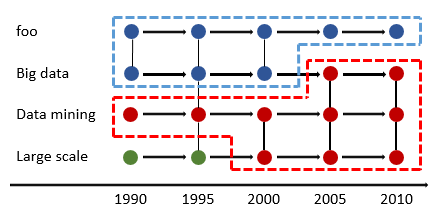
\includegraphics[width=0.80\linewidth]{figures/mutual.png}
\end{center}
There are two types of edges in the graph:

\begin{itemize}	
\item The concepts in the same time slide are connected with mutual info edge. For an arbitrary edge $(n_i^t, n_j^t)$, the weight from $n_i^t$ to $n_j^t$ is $W(n_i^t,n_j^t) = \frac{I(n_i^t,n_j^t)}{I(n_i^t,n_i^t)}$, where $I(n_i^t,n_j^t)$ indicates the mutual information between $w_i$ and $w_j$ within the time slide $t$.
\item Nodes corresponding to the term $w_i$ within two adjacent time slides $t$ and $t+1$ are connected by an evolving edge $(n_i^t,n_i^{t+1})$, indicates the knowledge concept is evolved from itself in the last time slide. The weight of the evolving edge is a parameter controlling the temporal smoothness of the summarization.
\end{itemize}

\textbf{Step.3 Knowledge concept selection}
The following task is to choose a set of terms best summarize the whole research area. We use two measures: \emph{Coverage} and \emph{Burstiness} to choose the terms of interest.

\begin{itemize}
\item We model burstiness by assuming the arrival of words as a unknown binomial distribution, and use $\chi^2$ tests to check for significant association between word and time periods. We calculate the contingency table as below and $\chi^2 = \frac{(ad-bc)^2n}{(a+b)(c+d)(a+c)(b+d)}$.
\begin{center}
\begin{tabularx}{0.5\linewidth}{ |X|X|X| }
  \hline
  - & $W$ & $\bar{W}$ \\
  \hline
  $t$  & a  & b  \\
  \hline
  $<t$  & c  & d  \\
  \hline
\end{tabularx}
\end{center}

\item We use a influence maximization based model to model information coverage of terms. More specifically, we use a linear threshold model, where influence probability from $n_i^t$ to $n_j^t$ is defined as $$P_{i,j}^{t} = \alpha P_{i,j}^{t-1} + (1-\alpha)W(n_i^t, n_j^t)}$$, and the activate threshold of $n_i^t$ is $$\Theta_i^t = \beta \Theta_i^{t-1} + (1-\beta) e^{\sum wX}$$, where $X$ is a feature vector and $w$ is the weight. The problem is to choose a set of $k$ term that maximize the content coverage. 

\end{itemize}

\textbf{Step.4 Trend partitioning}
After choosing a set of summarization words, we further grouping the rest of the words into clusters, and finally we can use the clusters over time to indict evolving trend and generates the highly intuitive visualization.


\section{Domain Knowledge}
\label{sec:approach}

The standard topic modeling techiques decomposing the observed data into latent topics according to a purely data-driven objective function. This means that topic models inherit some of the disadvantages of unsupervised learning. For example, there may be multiple candidate partitions of the dataset which capture different aspects of the underlying structure.

Purely unsuperivsed topic modeling discover topics which represent strong statistical patterns but do not always correspond to user expectations of semantically meaningful topics. 

Supervised LDA[Blei and McAuliffe, 2008] can be applied to labeled documents, augmenting each document $d$ with a label variable $y_d$, which either categorical or continuous. Each $y_d$ value is modeled by a Generalized Linear Model in the vector of mean topic counts $\bar{Z} = \frac{1}{N_d}\sum_{N_d}^{n=1}z_n$ for the document. This approach can therefore make label prediction by calculating the posterior topic assignments for a test document to obtain a $\bar{z}$ value. This model tends to produce topics that are able to "explain" the label value $y$ for the training set. In this way the label information indirectly influences the topic decomposion discovered by the model.

In dynamic topic models, the corpus is partitioned into disjoint time slices. Using logistic normal distributions, both the document-topic mixtures and topic-word multinomials evolve via multivariate Gaussian dynamics (i.e., at time step $s$ natural parameter $v_s$ is Gaussian distributed with mean $v_{s-1}$). Topics over time modeling timestamps as being genreated by the model itself. 

In standard LDA, topic-word multinomial distributions $\Phi_z = p(w|z)$ are drawn from a Dirichlet prior with hyperparameter $\beta$. To some extent, domain knowledge can be encoded into this Dirichlet prior by setting the values in the $\beta$ hyperparameter vector. The standard Dirichlet prior can be replaced with a more expressive Dirichlet Forest Prior.

The Dirichlet Tree distribution reparameterizes and generalized the standard Dirichlet distribution, while maintaining conjugacy to the multinomial. In the Dirichlet Tree, the leaf nodes correspond to the mulitnomial probabilities. The root node is assigned probability mass 1, which then "flows" to its children in proportion to a sample from Dirichlet distriution parametrized by the out-edge weights. Each internal node then distributes the probability mass it recives to its children in the same way.

The Dirichlet forest prior encodes both "Must-Link" and "Cannot-Link". It yeilds a mixture model of Dirichlet subtree within each connected component, each corresponds to a maximal clique. For each topic, one subtree is selected according to probability $$P(r) = |M_{rq}|, q = 1...Q^{(r)}.$$
Enssentially the selected subtree indexed by $q$ tends to redistribute nearly all probability mass to the words within $M_{rq}$. Since there is no mass left for other cliques, it is impossible for a word outside clique $M_{rq}$ to have a large probability. Therefore, no Cannot-Link will be violated.

LogicLDA allows the user to express domain knowledge in First-Order Logic. 
\begin{itemize}
\item \textbf{Constants} are symbols that represent an actual object in the problem domain.
\item \textbf{Variables} are symbols that can take on values from the set of constants.
\item \textbf{Predicates} are symbols that express relations, and evaluate to \emph{true} or \emph{false} for different arguments.
\item \textbf{Functions} are symbols that express mappings.
\item \textbf{Terms} are any expressions that refer to objects in the domain.
\item \textbf{Atoms} are predicates applied to terms.
\item \textbf{Formulas} are constructed from atoms using logical connectives $(\wedge,\vee,\neg,\Rightarrow)$.
\item \textbf{Clauses} are formulas consisting of a disjunction of literals.
\item \textbf{Ground} terms, atoms, or formulas contain no variables.
\end{itemize}

Markov Logic Networks are a class of graphical models operate over this type of logical domain. A "possible world" consists of a set of binary assignments for all possible ground predicates. A MLN then assigns probabilities to all possible worlds. 

\begin{itemize}
\item $Z(i,t)$ is true if the hidden topic $z_i = t$, and false otherwise.
\item $W(i,v)$ is true if word $w_i = v$, and false otherwise.
\item $D(i,j)$ is true if $d_i = j$, and false otherwise.
\end{itemize}

The model probability of LogicLDA can be interpreted as the product of the individual MLN and LDA contributions. Another perspective is that LogicLDA consists of an MLN augmented with continuous varibles $(\Theta, \Phi)$ and associated potential functions.

The goal of LogicLDA is to learn the most likely $\phi$ and $\theta$ in the model. As in standard LDA, the latent topic assignment $z$ cannot be marginalized out in practice due to their combinatorial nature. We instead aim to find the maximum a posteriori estimate of $z$, $\Theta$, $\Phi$ jointly. This can be formulated as maximizing the logarithm of the unnormalized probability.
\section{Summarization Framework}
\label{sec:algorithm}

The major motivation of our work is to find a concise and intuitive summarization of a given research topic. More concretely, we want to select a set of representative terms that best describe the hot spots and major achievements along the development of the research topic, meanwhile, capture the temporal evolutionary pattern within the research area. We formulated the problem as a graph partitioning task. At a high level, the proposed summarization framework consists of three stages.

\begin{itemize}
    \item {\bf Document retrieval.} First, given a research topic $q$ needs to be summarized, we find a documents collection $D = \{d_t\}^T$ that can represent the development of the research topic, where $d_t$ denote the documents at time $t$.
    
    \item {\bf Dynamic concept graph construction.}  
    Second, we extract knowledge concept terms mentioned in each document and construct a graph $G$, where each term $w_i$ at time slide $t$ is associated with a node $n_i^t$. We explicitly model the semantic relationship and evolving patterns with the graph by associating feature scores on the nodes and edges.
    
    \item {\bf Trend partitioning.} Third, we utilize a message passing algorithm on the constructed dynamic concept graph to select a set of terms based on their \emph{authority}, \emph{burstiness} and network structures, and further partition the graph into evolutionary trends.
\end{itemize}

\subsection{Document Retrieval}

To summarize a given research topic $t$ (i.e., user's query), we need to first map the topic to a set of documents. A straightforward idea is to use some traditional information retrieval technique to find the relevant documents. However, such an approach is not appropriate for the dynamic summarization task due to the following reasons. First, we want to summarize the development of the topic over time, if we use such an approach, we won't be able to trace how a knowledge concept evolve from and emerge into some other related concepts. Second, it has obvious bias that most retrieved documents will contain the queried words. Third, if a query contains a rare used term or a new term, it will face the problem of data sparseness. 

To overcome the disadvantages above, we use a community-base document retrieval method. We first find a core research community (a group of experts) related to the topic, and then aggregate all the members' research work as the document collection to summarize. Such an approach is very intuitive since these researchers are leading the development the research area. To avoid some authoritative experts' work dominated in the documents and introduce potential bias, we normalize each member's contribution averagely.

\subsection{Dynamic Concept Graph Construction}
After the initial retrieval of related document collection, we extract knowledge concepts mentioned in each documents. In this work, we simply use wikipedia titles as a vocabulary to extract terms. With the extracted terms of each document over time, we construct a dynamic concept graph $G=\{V,E_r,E_e\}$ to model the semantic relationship and evolutionary pattern between terms uniformly. For a term $w_i$, we create a node $n_i^t$ for each time slide $t$. There are two types of edges in the graph, $E_r$ are representative edges denotes how well-suited for a term to act as a representative of another term at a given time. $E_e$ are evolving edges connecting the same terms within two adjacent time slides indicating to what extent the meaning of the term has shifted.

\begin{center}
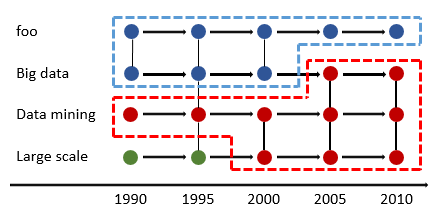
\includegraphics[width=0.80\linewidth]{figures/mutual.png}
\end{center}

\begin{itemize}

\item \textbf{Representativeness:} 
To capture the semantic relationship between terms, we connect terms co-occurred in the documents at the same time slide with representative edges. Formally, the weight of the directed edge $(n_i^t,n_j^t)$ is defined based on mutual information, indicates how appropriate it is to use term $w_i$ to represent $w_j$ at time $t$. We calculate mutual information between term $w_i$ and term $w_j$ at the given time slide $t$ as:
\begin{equation}
\begin{split}
I(n_i^t,n_j^t) & = p(w_i \in d_t, w_j \in d_t)log{\frac{p(w_i\in d_t, w_j \in d_t)}{p(w_i \in d_t)p(w_j \in d_t)}} \\
& + p(w_i \in d_t, w_j \notin d_t)log{\frac{p(w_i\in d_t, w_j \notin d_t)}{p(w_i \in d_t)p(w_j \notin d_t)}} \\
& + p(w_i \notin d_t, w_j \in d_t)log{\frac{p(w_i\notin d_t, w_j \in d_t)}{p(w_i \notin d_t)p(w_j \in d_t)}} \\
& + p(w_i \notin d_t, w_j \notin d_t)log{\frac{p(w_i\notin d_t, w_j \notin d_t)}{p(w_i \notin d_t)p(w_j \notin d_t)}}
\end{split}
\end{equation}

where $d_t$ denotes all the retrieved documents at time $t$. The representativeness of term $w_i$ to term $w_j$ at time $t$ is then defined as normalized mutual information $$s(n_i^t,n_j^t) = \frac{I(n_i^t,n_j^t)}{I(n_i^t,I_i^t)}$$


\item \textbf{Meaning shift:}
Nodes corresponding to the term $w_i$ within two adjacent time slides $-1t$ and $t$ are connected by an evolving edge $(n_i^{t-1},n_i^{t})$, indicates that the term is evolved from itself at the last time slide. The weight of the evolving edge indicates whether the meaning of the term is staying the same or shifted from time $t-1$ to $t$. Formally the weight is defined based on Jaccard coeffient.
$$s(n_i^{t-1},n_i^t) = \frac{|NB(n_i^{t-1}) \cap NB(n_i^t)|}{|NB(n_i^{t-1}) \cup NB(n_i^t)|}$$

\item \textbf{Burstiness:}
We model burstiness by assuming the arrival of terms as an unknown binomial distribution, and use $\chi^2$ tests to check for significant association between words and time periods. We calculate the contingency table as below and $\chi^2 = \frac{(ad-bc)^2n}{(a+b)(c+d)(a+c)(b+d)}$.
\begin{center}
\begin{tabularx}{0.5\linewidth}{ |X|X|X| }
  \hline
  - & $W$ & $\bar{W}$ \\
  \hline
  $t$  & a  & b  \\
  \hline
  $<t$  & c  & d  \\
  \hline
\end{tabularx}
\end{center}

We define burstiness of term $w_i$ at time $t$ as $b_i^t = \chi^2$ value.

\item \textbf{Authority:}
We simply defined the authority of a term at a given time by $u_i^t=df_t(w_i)/|d_t|$, where $df_t(w_i)$ indicates the document frequency of $w_i$ at time $t$, and $|d_t|$ is the number of documents at time $t$.
\end{itemize}




\subsection{Trend Partitioning}
In order to give a concise and intuitive summarization, we need to partition the dynamic concept graph into evolutionary trends, and select a set of representative terms best describe the development of the research topic. Here, we use a massage passing algorithm to perform the selection and partition. The method is analogous to affinity propagation(AP) algorithm proposed in Frey et al. and Tang et al, the difference is that our method is modified to fit the dynamic setting. The AP algorithm performs clustering by identifying exemplars. Essentially it solves the following optimization problem
$$c^* = argmin(-\sum S(i,c_i) )$$
where $C=(c_i)$ is the mapping between nodes and exemplars, $S(i,c_i)$ indicates the similarity between $i$ and its exemplar. $S(i,i)$ is the penalty for i to being exemplar of itself.

In the algorithm, we introduce three sets of variables $\{r_{ij}^t\}$, $\{a_{ij}^t\}$ and $\{e_i^{t-1,t}\}$. Where $r_{ij}^t$ indicates the how well-suited term $w_j$ is to serve as an exemplar of term $w_i$ (i.e. $w_j$ covers the meaning of $w_i$) at time slide $t$. $a_{ij}$ denotes the availabilities of term $w_j$ to serve as an exemplar of $w_i$ at time $t$. $\{e_i^{t-1,t}\}$ indicates the equivalence between the term $w_i$ at two adjacent time slides which captures to what extent the meaning of term $w_i$ has shifted from $t-1$ to $t$.
All the $r_{ij}^t$, $a_{ij}^t$ and $e_i^{t-1,t}$ are set to $0$ initially, their values are updated iteratively with following rules until convergence.
\beal{
r_{ij}^t = (1-\lambda)\rho_{ij}^t+\lambda r_{ij}^t\\
a_{ij}^t = (1-\lambda)\alpha_{ij}^t+\lambda a_{ij}^t
}
where $\lambda$ is a damping factor, $\rho_{ij}^t$ and $\alpha_{ij}^t$ are messages passing from $n_i^t$ to $n_j^t$. The massage passing rules are defined as follows:


\beal{
\rho_{ij}^t = s(n_i^t,n_j^t) - \max_{k\in NB(n_j^t)}\{s(n_i^t,n_k^t) + a_{ik}^t\}\\
\alpha_{ii}^t = \sum_{k\in NB(n_i^t)}\max\{0,r_{ij}^t\}\\
\alpha_{ij}^t = min\{0,r_{jj}^t + \sum_{k \in NB(n_j^t)}\max\{0,r_{ik}^t\}\}
}

\begin{algorithm}[t]
\label{alg:learning}
\caption{Message passing algorithm on dynamic concept graph.}
\small
% factor graph learning
%Learning step:
%\BlankLine
\SetLine \KwIn{dynamic concept graph $G=\{V,E_r,E_e\}$;}
\KwOut{a set of representative nodes $V_r$ and the par;}
%// Generate train data\;
%$G=\emptyset$\;
Initialize all ${r_{ij}^t}\leftarrow\mathbf{0}$\;
\Repeat{converge}{
    \ForEach{edge ($n_i^t$)}{
     //Initialization\;
    $L \leftarrow$ initialization list\;
    %$inventorction(L)$\;
    %$L \leftarrow RemoveUnlabelNodes(L)$\;

%\BlankLine
Factor graph $FG \leftarrow BuildFactorGraph(L)$\;

// Learn the parameter $\mathbf{\theta}$ for factor graph model\;
%$order \leftarrow BuildUpdateOrder(FG)$\;

\Repeat{(all messages $\mu$ do not change)}{
    \ForEach {$v_i \in order$} {
        Update the messages of $v_i$\ by Eqs.~\ref{eq:sp_v} and \ref{eq:sp_f};
    }
}
\ForEach{$\theta_i\in \mathbf{\theta}$} {
    Calculate gradient $\nabla_i$ according to Eq. \ref{eq:gradient}\;
    Update $\theta^{new} = \theta^{old} + \eta \cdot \nabla_i$\;
}
}
}
\normalsize
\end{algorithm}

where $NB(n_j^t)$ denotes the neighboring nodes of node $n_j^t$, $s(n_i^t,n_j^t)$ is $w_i$'s representativeness of $w_j$ at time $t$. $s(n_i^t,n_i^t)$ is set to $s(n_i^t,n_i^t) = \beta b_i^t + (1-\beta)u_i^t$ indicates that the nodes with high authority and burstiness are preferred to be choose as exemplars, where $\beta$ is a parameter controlling the trade-off between timeliness and importance. 




%\input{observation.tex}
%\input{exp.tex}
%\input{exp_new.tex}
%\section{Related Works}
\label{sec:related}

%\section{Conclusion}
\label{sec:conclusion}



%\small
\bibliographystyle{abbrv}
%\bibliography{references-full}
% sigproc.bib is the name of the Bibliography in this case
\begin{thebibliography}{10}


\end{thebibliography}

\normalsize

\end{document}
